\documentclass[11pt,ignorenonframetext,]{beamer}
\usetheme{Boadilla}
\usepackage{amssymb,amsmath}
\usepackage{ifxetex,ifluatex}
\ifxetex
  \usepackage{fontspec,xltxtra,xunicode}
  \defaultfontfeatures{Mapping=tex-text,Scale=MatchLowercase}
\else
  \ifluatex
    \usepackage{fontspec}
    \defaultfontfeatures{Mapping=tex-text,Scale=MatchLowercase}
  \else
    \usepackage[utf8]{inputenc}
  \fi
\fi
\usepackage{enumerate}
\usepackage{graphicx}
% Comment these out if you don't want a slide with just the
% part/section/subsection/subsubsection title:
\AtBeginPart{\frame{\partpage}}
\AtBeginSection{\frame{\sectionpage}}
\AtBeginSubsection{\frame{\subsectionpage}}
\AtBeginSubsubsection{\frame{\subsubsectionpage}}
\setlength{\parindent}{0pt}
\setlength{\parskip}{6pt plus 2pt minus 1pt}
\setlength{\emergencystretch}{3em}  % prevent overfull lines
\setcounter{secnumdepth}{0}

\title[A Short Introduction to git]{Learning by Doing}
\subtitle{\href{https://github.com/weijianwen/GitForBeginners}{{A Short Introduction to git}}}
\author{Jianwen WEI}
\institute[SJTU]{Shanghai Jiaotong University}
\date{\today}

\begin{document}
\frame{\titlepage}

\begin{frame}
       \frametitle{Outline}
       \tableofcontents
\end{frame}

\section{What is git?}

\begin{frame}\frametitle{What does a
\href{http://en.wikipedia.org/wiki/Revision\_control}{Version Control System} 
do?}

\begin{columns}
  \begin{column}{0.7\textwidth}
\begin{itemize}
\item
  Track source code
  \begin{itemize}
  \item
    Maintain code history, integrity, atomic change\ldots{}
  \end{itemize}
\item
  Coordinate distributed development
  \begin{itemize}
  \item
    branch, merge conflicts, tag\ldots{}
  \end{itemize}
\end{itemize}

 \end{column}

  \begin{column}{0.3\textwidth}
 \begin{figure}[htbp]
\centering
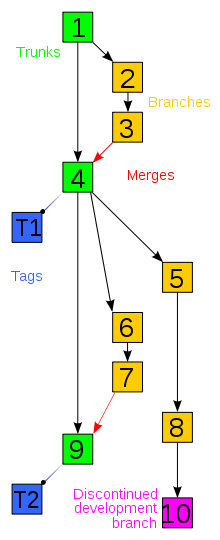
\includegraphics[width=0.85\textwidth]{figures/vcsflow.png}
\caption{VCS work flow}
\end{figure}
  \end{column}
\end{columns}
\bigskip

\end{frame}


\begin{frame}\frametitle{VCS Work Flow Categories}

\begin{itemize}
\item
  Centralized:
  \href{http://msdn.microsoft.com/en-us/library/3h0544kx(v=vs.80).aspx}{VSS},
  \href{http://www.nongnu.org/cvs/}{CVS},
  \href{http://subversion.apache.org/}{SVN}
\item
  Distributed\footnote{Distributed VCSs support centralized work flow
    too.}: \href{http://www.bitkeeper.com/}{BitKeeper},
  \href{http://git-scm.com/}{git},
  \href{http://mercurial.selenic.com/}{mercurial}\ldots{}
\end{itemize}
\end{frame}

\begin{frame}\frametitle{Why git is better than X (SVN, CVS, \ldots{})}

\begin{itemize}
\item
  git is super fast
\item
  Full repository clone
\item
  Local history: no need to connect to servers when viewing the revision
  history
\item
  Cheap branch and easy merge
\item
  \href{https://github.com/}{github}: social coding\footnote{\href{https://bitbucket.org}{bitbucket},
    \href{http://code.google.com}{Google Code} support git too, but
    github in no doubt has more
    \href{http://shop.github.com/}{\emph{fun}}.}
\item
  Other things: tidy working directory, better compression, multi work
  flow support, \ldots{}
\end{itemize}
\end{frame}

\begin{frame}\frametitle{General Advice on Learning git}

\begin{itemize}
\item
  Try git and github
\item
  Most graphical tool/plug-ins\footnote{\href{http://code.google.com/p/tortoisegit/}{tortoisegit},
    \href{http://lostechies.com/joshuaflanagan/2010/09/03/use-gitk-to-understand-git/}{gitk},
    \href{http://www.eclipse.org/egit/}{EGit},
    \href{https://github.com/blog/1067-github-for-mac-1-2-snow-octocat}{Snow
    Octocat}\ldots{} But please, oh please use the command-line tool.}
  \emph{SUCK}. Please use the command-line git.
\item
  Read git's prompts, run \textbf{git help} to get help.
\item
  Find ``how-to'' on Google, StackOverflow, git book.
\end{itemize}
\end{frame}

\begin{frame}\frametitle{Rules of Thumb for git}

\begin{itemize}
\item
  ``A clear development flow is worth thousands of VCSs.''
\item
  Modular design, avoid simultaneous source file editing by different
  members.
\item
  Head version at trunk is always ready to deploy.
\item
  Modification is made on branches, then merged into trunk.
\item
  Stay on your own branch.
\item
  Write comment to each commit.
\end{itemize}
\end{frame}

\section{Learning and USING git}

\begin{frame}\frametitle{To get started, I will\ldots{}}

\begin{itemize}
\item
  Illustrate git's various work flows.
\item
  Explain the most frequently used git commands.
\item
  Give exercises for self check. Some of the exercises require github
  access.
\end{itemize}
\end{frame}

\begin{frame}\frametitle{git's stand-alone work flow}

\begin{itemize}
\item
  You can use git on a stand-alone computer and easily integrate the
  code into a more sophisticated work flow (distributed or centralized)
  at a later time.
\end{itemize}
\begin{figure}[htbp]
\centering
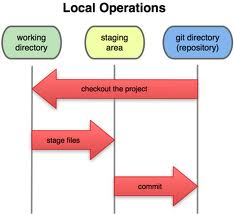
\includegraphics[width=0.45\textwidth]{figures/gitstandalone.jpeg}
\caption{git's local work flow}
\end{figure}

\end{frame}

\begin{frame}\frametitle{git's distributed work flow}

\begin{itemize}
\item
  Every collaborator keeps a full clone of the repository.
\item
  All repositories are peers.
\item
  Repositories are not necessarily consistent at all time. Use push/pull
  to exchange changes when necessary.
\end{itemize}
\begin{figure}[htbp]
\centering
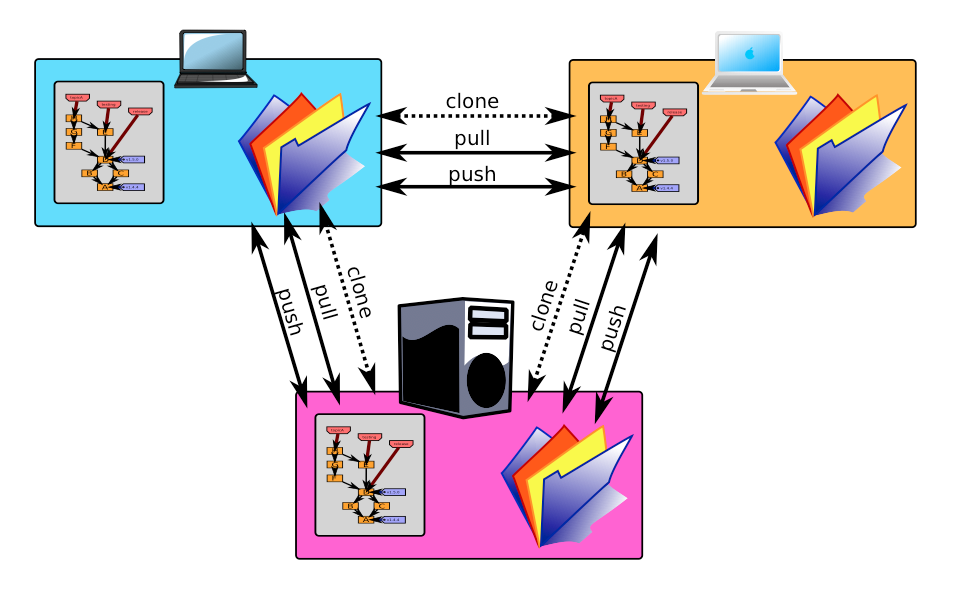
\includegraphics[width=0.6\textwidth]{figures/gitdvcs.png}
\caption{git's distributed work flow}
\end{figure}

\end{frame}

\begin{frame}\frametitle{git's emulation to the centralized work flow
(\textbf{RECOMMENDED})}

\begin{columns}
	\begin{column}{0.6\textwidth}
	\begin{itemize}
	\item It's \textbf{emulation}, not \emph{real}.
	\item The statement, ``all repositories are peers.'', still holds.
	\item We pretend that we see the central repo only, unaware of each other's peer repo.
	\end{itemize}
	\end{column}

	\begin{column}{0.4\textwidth}
	\begin{figure}[htbp]
	\centering
	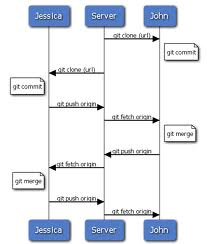
\includegraphics[width=0.9\textwidth]{figures/gitcent.jpeg}
	\caption{git's centralized work flow for John and Jessica}
	\end{figure}
	\end{column}
\end{columns}

\end{frame}

\begin{frame}[fragile]\frametitle{Set up git}

\begin{itemize}
\item
  Please follow github's nice tutorials to set up\footnote{The email you
    fill in when signing up is used for web login and password reset
    only. github uses SSH keys for \texttt{git} authentication. Try to
    clarify the following \emph{pass phrases}: your email account's pass
    phrase, your github account's pass phrase, and the pass phrase to
    access your SSH private key.} git on
  \href{http://help.github.com/win-set-up-git/}{Windows},
  \href{http://help.github.com/linux-set-up-git/}{Linux} or
  \href{http://help.github.com/mac-set-up-git/}{Mac}.
\item
  \href{http://linux.vbird.org/linux\_server/0310telnetssh.php\#ssh\_server}{Must-known
  things about SSH keys}: private key, public key, the pass phrase to
  access the private key, key fingerprint.
\item
  Don't forget to set \texttt{user.name} and
  \texttt{user.email}\footnote{Usernames and emails in git's
    configuration are for identification purpose only, not for sending
    emails. It is highly recommended that the email in git and SSH keeps
    the same.} before your very first git commit.
\end{itemize}
\end{frame}

\begin{frame}\frametitle{git command}

\begin{itemize}
\item
  help
\item
  init
\item
  status
\item
  add
\item
  commit
\item
  diff
\item
  tag
\item
  Working with branch
\item
  Working with remotes
\item
  submodule
\item
  Oh, there is a conflict!!!
\item
  ``Time Machine''
\end{itemize}
\end{frame}

\begin{frame}[fragile]\frametitle{\texttt{help}: Get help}

\texttt{git help COMMAND} Get help from git.

\begin{itemize}
\item
  \texttt{git help add}
\item
  \texttt{git help commit}
\item
  \ldots{}
\end{itemize}
\end{frame}

\begin{frame}[fragile]\frametitle{\texttt{init}: Initialize a local git
repo for your project}

\texttt{init} command will create a \texttt{.git} dir on the top level
of your project.

\begin{enumerate}[1.]
\item
  \texttt{cd YOUR\_PROJ\_DIR}
\item
  \texttt{git init .}
\end{enumerate}
\end{frame}

\begin{frame}[fragile]\frametitle{\texttt{status}: Show the status of
your repo}

\texttt{git status}

\begin{itemize}
\item
  \texttt{status} tells you how to \textbf{UNDO} the last operation on
  git
\item
  \href{http://progit.org/book/ch2-2.html}{File status}:
  \texttt{untracked}, \texttt{unstaged}, \texttt{staged} (indexed),
  \texttt{committed}\footnote{The \emph{committed} status simply
    displays nothing when running \texttt{git status}.}
\end{itemize}
\begin{figure}[htbp]
\centering
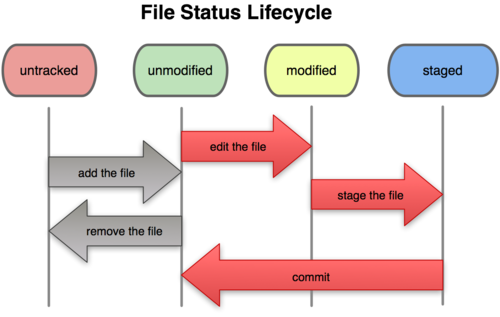
\includegraphics[width=0.5\textwidth]{figures/gitlifecycle.png}
\caption{File Status Lifecycle}
\end{figure}

\end{frame}

\begin{frame}[fragile]\frametitle{\texttt{add}: A multi-function git
command}

\texttt{git add FILES\_OR\_DIR}

\begin{itemize}
\item
  For untracked files: \emph{add} them to git's control
\item
  For unstaged changes: \emph{add} them to the staged area
\item
  For conflicted files: \emph{add} marks them as ``resolved''
\end{itemize}
\end{frame}

\begin{frame}[fragile]\frametitle{commit: Store the status (snapshot)
permanently}

\begin{itemize}
\item
  \texttt{git commit -m "YOUR\_COMMENT"}
  \begin{itemize}
  \item
    \texttt{git commit} Stores the STAGED changes only
  \item
    \texttt{git commit -a} Stores all the STAGED and UNSTAGED changes.
  \end{itemize}
\item
  Please write comment for each of your commit.
\item
  Each commit is identified by a \textbf{UNIQUE} SHA-1 ID of 40 ASCII
  characters.
\end{itemize}
\begin{verbatim}
     commit dd5f924c40096b9cda27ffd1cfd1205822ab3c70
     Author: Github Support <me@github.com>
     Date:   Sun Apr 1 19:38:37 2012 +0800

        Restart the git-tutorial project.
\end{verbatim}
\end{frame}

\begin{frame}[fragile]\frametitle{diff: Find differences}

\begin{itemize}
\item
  \texttt{git diff}
  \begin{itemize}
  \item
    changes between the staged and working files
  \end{itemize}
\item
  \texttt{git diff -{}-staged}
  \begin{itemize}
  \item
    changes between the HEAD and the staged files
  \end{itemize}
\item
  \texttt{git diff HEAD}
  \begin{itemize}
  \item
    changes between the HEAD and the working files
  \end{itemize}
\item
  \texttt{git diff COMMIT\_ID COMMIT\_ID}
  \begin{itemize}
  \item
    changes between two commits
  \end{itemize}
\end{itemize}
\end{frame}

\begin{frame}[fragile]\frametitle{tag: A milestone version}

\begin{itemize}
\item
  \texttt{git tag}
  \begin{itemize}
  \item
    See all the tag
  \end{itemize}
\item
  \texttt{git show TAG\_NAME}
  \begin{itemize}
  \item
    See a tag in detail
  \end{itemize}
\item
  \texttt{git tag TAG\_NAME}
  \begin{itemize}
  \item
    Add a ``lightweight'' tag
  \end{itemize}
\item
  \texttt{git tag -a TAG\_NAME -M YOUR\_COMMENT}
  \begin{itemize}
  \item
    Add an annotated tag
  \end{itemize}
\item
  \texttt{git tag -d TAG\_NAME}
  \begin{itemize}
  \item
    Delete a tag
  \end{itemize}
\end{itemize}
\end{frame}

\begin{frame}[fragile]\frametitle{Submodule: Integrate multi git repos}

\begin{itemize}
\item
  \texttt{git help submodule}
\item
  \href{http://progit.org/book/ch6-6.html}{Repo in Repo}
\item
  Manage other repos as ``submodules'' in your project
\end{itemize}
\end{frame}

\begin{frame}\frametitle{Working with \textbf{branch}: branch, checkout,
merge}

A branch-based development flow:

\begin{enumerate}[1.]
\item
  Create a branch
\item
  Switch to the newly-created branch
\item
  Modify and commit on the branch
\item
  Merge branch's changes into trunk.
\end{enumerate}
\end{frame}

\begin{frame}[fragile]\frametitle{Working with \textbf{branch}:
\texttt{branch}, checkout, merge}

\begin{itemize}
\item
  \texttt{git branch} See all the branches
\item
  \texttt{git branch BRANCH\_NAME} Create a branch
\item
  \texttt{git branch -d BRANCH\_NAME} Delete a branch
\item
  \texttt{git branch -D BRANCH\_NAME} Force delete a branch
\end{itemize}
\end{frame}

\begin{frame}[fragile]\frametitle{Working with \textbf{branch}: branch,
\texttt{checkout}, merge}

\begin{itemize}
\item
  \texttt{git checkout BRANCH\_NAME} Switch to a branch. The working
  files will change.\footnote{Don't confuse git's term \texttt{checkout}
    here with Subversion's checkout.}
\item
  \texttt{git checkout -f BRANCH\_NAME} Force switch to a branch
\item
  \texttt{git checkout master} Go back to trunk, named \emph{master} in
  git.
\item
  \texttt{git checkout -b BRANCH\_NAME} Create a branch then switch to
  it.
\end{itemize}
\end{frame}

\begin{frame}[fragile]\frametitle{Working with \textbf{branch}: branch,
checkout, \texttt{merge}}

\begin{itemize}
\item
  \texttt{git merge BRANCH\_A BRANCH\_B} Merge branch\_a's and
  branch\_b's changes into \emph{current} branch
\item
  \texttt{git checkout master, git merge master BRANCH\_NAME} Merge
  changes into trunk, the master branch.
\end{itemize}
\end{frame}

\begin{frame}[fragile]\frametitle{Working with \textbf{remotes}:
\texttt{clone}, remote, push, pull}

\begin{itemize}
\item
  \texttt{git clone REPO\_URL} Full clone of a repo.
\item
  URL can be in forms of local dir (\textasciitilde{}/proj), git
  (git://xxx), SSH (ssh://xxx), https (http://xxx)\ldots{}
\end{itemize}
\end{frame}

\begin{frame}[fragile]\frametitle{Working with \textbf{remotes}: clone,
\emph{remote}, push, pull}

\begin{itemize}
\item
  \texttt{remote} Manages the set of tracked repositories.\footnote{Remote
    repos in git are just references or pointers, so you lose or gain
    \emph{nothing} when adding or removing a remote repo.}
\item
  \texttt{git remote}
  \begin{itemize}
  \item
    Show all the tracked repositories.
  \end{itemize}
\item
  \texttt{git remote show REPO\_NAME}
  \begin{itemize}
  \item
    Show the repo's details.
  \end{itemize}
\item
  \texttt{git remote add REPO\_NAME REPO\_URL}
  \begin{itemize}
  \item
    Add a remote repo to tracked list.
  \end{itemize}
\item
  \texttt{git remote -d REPO\_NAME}
  \begin{itemize}
  \item
    Remove a remote repo from the tracked list.
  \end{itemize}
\item
  \texttt{git remote rename REPO\_OLD REPO\_NEW}
  \begin{itemize}
  \item
    Rename a repo.
  \end{itemize}
\end{itemize}
\end{frame}

\begin{frame}[fragile]\frametitle{Working with \textbf{remotes}: clone,
remote, \emph{push, pull}}

\begin{itemize}
\item
  \texttt{git pull REPO\_NAME REMO\_BRANCH}
  \begin{itemize}
  \item
    Merge remote branch's changes into current branch.
  \end{itemize}
\item
  \texttt{git push REPO\_NAME REMO\_BRANCH}
  \begin{itemize}
  \item
    Push current branch's changes to the remote branch.
  \end{itemize}
\item
  \texttt{git push REPO\_NAME :REMO\_BRANCH}
  \begin{itemize}
  \item
    Delete a remote branch.
  \end{itemize}
\end{itemize}
\end{frame}

\begin{frame}[fragile]\frametitle{Oh, there is a conflict!!!}

\begin{itemize}
\item
  A conflict looks like:
\end{itemize}
\texttt{\textless{}\textless{}\textless{}\textless{}\textless{}\textless{}\textless{} HEAD:index.html \textless{}div id="footer"\textgreater{}contact : email.support@github.com\textless{}/div\textgreater{} ======= \textless{}div id="footer"\textgreater{}   please contact us at support@github.com \textless{}/div\textgreater{} \textgreater{}\textgreater{}\textgreater{}\textgreater{}\textgreater{}\textgreater{}\textgreater{} iss53:index.html}

\begin{itemize}
\item
  Conflicts arise when git cannot automatically merge changes at
  \texttt{merge} or \texttt{pull} operations.
\item
  Don't panic. Conflicts are no big deal, sometimes even inevitable.
\item
  What you should do: merge the conflicts, mark the files as
  ``resolved'', then commit the changes.
\end{itemize}
\end{frame}

\begin{frame}[fragile]\frametitle{Working with conflicts: merge,
resolve, commit}

\begin{enumerate}[1.]
\item
  You have to edit the conflicted files, merge conflicts MANUALLY.
  \texttt{diff} command may help you.
\item
  \texttt{git add CONFLICT\_FILES} Mark the file as resolved.
\item
  \texttt{git commit -m "YOUR\_COMM"} Commit changes to the repo.
\end{enumerate}
\end{frame}

\begin{frame}[fragile]\frametitle{``Time Machine'': \texttt{stash},
checkout}

\texttt{stash} saves your temporary work and resets the files to HEAD
version. You can handle some emergency fix first then continue to hack
at a latter time.

\begin{enumerate}[1.]
\item
  \texttt{git stash}
  \begin{itemize}
  \item
    Save the temp changes.
  \end{itemize}
\item
  \texttt{git stash list}
  \begin{itemize}
  \item
    Check the stash list.
  \end{itemize}
\item
  EDIT and COMMIT your emergency fix.
\item
  \texttt{git stash pop}
  \begin{itemize}
  \item
    Continue to hack
  \end{itemize}
\end{enumerate}
\end{frame}

\begin{frame}[fragile]\frametitle{``Time Machine'': stash,
\texttt{checkout}}

\texttt{checkout} enable you to go backward and forward in the revision
history.

\begin{enumerate}[1.]
\item
  \texttt{git checkout COMMITID\_OR\_TAGNAME} \footnote{The full commit
    ID is 40 characters long. But you may type a short prefix (like
    4\textasciitilde{}6 characters) to refer a commit uniquely.}
  \begin{itemize}
  \item
    Time Machine starts up.
  \end{itemize}
\item
  You are on a \texttt{unnamed} branch with file status dating back. Do
  anything you want.
\item
  \texttt{git checkout master}
  \begin{itemize}
  \item
    Come back to master.
  \end{itemize}
\end{enumerate}
\end{frame}

\section{Exercises}

\begin{frame}[fragile]\frametitle{Exercise: Set up git environment}

\begin{enumerate}[1.]
\item
  Set up git on your computer, and sign up a github account.
\item
  Initialize a local project as git repo, make your first git.
\item
  Email your SSH public key file as an attachment to
  \href{mailto:weijianwen@sjtu.edu.cn}{me}. Name your pubkey file after
  ``YOUR@EMAIL.pub'', e.g., you should rename your \texttt{id\_rsa.pub}
  to \texttt{xxx@sjtu.edu.cn.pub} and send it to me.
\end{enumerate}
\end{frame}

\begin{frame}[fragile]\frametitle{Exercise: git basics}

Be familiar with \texttt{status}, \texttt{add}, \texttt{commit},
\texttt{diff}, \texttt{tag}.

\end{frame}

\begin{frame}\frametitle{Exercise: Branch-based development}

\begin{enumerate}[1.]
\item
  Create a branch.
\item
  Checkout to that branch.
\item
  Merge the changes into trunk (master).
\item
  Delete the branch.
\end{enumerate}
\end{frame}

\begin{frame}[fragile]\frametitle{Exercise: Be social on github}

\begin{enumerate}[1.]
\item
  Follow \href{https://github.com/weijianwen}{me} on github.\footnote{Please
    feel free to unfollow me when finishing all the required exercises.}
\item
  I will add you as a collaborator. Please wait for my message on github
  before proceeding to next step.
\item
  Clone the
  \href{https://github.com/weijianwen/GitForBeginners}{GitForBeginners}
  project with Read+Write access.
\item
  Write something into the \texttt{README.txt} (DON'T destroy the
  description header). add, commit, pull, push.
\end{enumerate}
\end{frame}

\begin{frame}[fragile]\frametitle{Exercise: Manage remotes}

\begin{enumerate}[1.]
\item
  You clone the remote repo
  \href{https://github.com/weijianwen/GitForBeginners}{GitForBeginners}
  on github. Try \texttt{git remote}.
\item
  Copy the
  \href{git@github.com:weijianwen/GitForBeginners.git}{REPO\_URL} to
  somewhere else.
\item
  Delete the remote repo.\footnote{Don't worry. It is just a reference.}
\item
  Add the remote repo
  \href{git@github.com:weijianwen/GitForBeginners.git}{REPO\_URL} with a
  name you prefer, such as \texttt{myrepo}.
\item
  Rename the remote repo to its original name -- \texttt{origin}.
\end{enumerate}
\end{frame}

\begin{frame}[fragile]\frametitle{Exercise: Remote branch}

\begin{enumerate}[1.]
\item
  Create a local branch with your full name, such as \texttt{zhangsan}.
\item
  Write something into README.txt on the branch. add, commit, pull, push
  to the remote branch.
\item
  Leave the branch on github as a mark of ``I finish the homework''.
  Please recreate the remote branch if you've tried the \emph{delete
  remote branch} command.
\end{enumerate}
\end{frame}

\begin{frame}[fragile]\frametitle{Exercise: Handle conflicts}

\begin{enumerate}[1.]
\item
  Clone
  \href{https://github.com/weijianwen/GitForBeginners}{GitForBeginners}
  twice into two separate projects, namely \texttt{proj\_A} and
  \texttt{proj\_B}.
\item
  In proj\_A, modify README.txt. add, commit, pull, push
\item
  In proj\_B, modify the \emph{SAME} lines of README.txt as you do in
  proj\_A. add, commit, pull
\item
  A \emph{conflict} towards README.txt arises in proj\_B.
\item
  Resolve the conflict, then add, commit, pull, push to github.
\end{enumerate}
\end{frame}

\begin{frame}[fragile]\frametitle{Exercise: Time Machine}

Use \texttt{stash}, \texttt{checkout} to do time travel.

\end{frame}

\section{Recommended Materials}

\begin{frame}\frametitle{Recommended Materials for Learning git}

\begin{itemize}
\item
  \href{http://goo.gl/NBGgo}{``Git Tutorials'' by Li Yanrui}
\item
  \href{http://help.github.com/}{github:help}
\item
  \href{http://progit.org/book/}{Pro Git On line}
\item
  \href{http://excess.org/article/2008/07/ogre-git-tutorial/}{Video:
  ``Git the basics'' by Bart Trojanowski}
\item
  \href{http://shop.oreilly.com/product/0636920022862.do}{O'Reilly Book:
  Version Control With Git, 2nd Edition}
\end{itemize}
\end{frame}

\end{document}
